\documentclass{letter}

\usepackage[left=0.75in, right=0.75in, top=1.1in, bottom=0.75in]{geometry}
\usepackage{fancyhdr, amsmath, amssymb, mathtools, xcolor, graphicx, listings, mathpazo}
\graphicspath{{.}}

\pagestyle{fancy}
\fancyhf{}
\rhead{Page \thepage}
\chead{AMSC808N Homework 3}
\lhead{Tyler Hoffman}
\setlength{\headsep}{0.2in}

\newcounter{problem}
\newcounter{subproblem}[problem]
\newcounter{solution}

\renewcommand{\thesubproblem}{(\alph{subproblem})}

\newcommand{\Problem}[2]{%
	\stepcounter{problem}%
	\leftskip=0pt%
	\theproblem.~\textbf{{#1.}} #2 \par%
}

\newcommand{\Subproblem}[1]{%
	\stepcounter{subproblem}%
	\leftskip=15pt%
	\thesubproblem~ #1 \par%
}

\newcommand{\Solution}[1]{%
	\textbf{Solution.} #1 \par%
}

\newcommand{\Due}[1]{\textbf{Due: #1} \par}

\newcommand{\UNFINISHED}{\textbf{\color{red} UNFINISHED}}
\newcommand{\CHECK}{\textbf{\color{orange} CHECK ME}}

\newcommand{\iu}{{i\mkern1mu}}
\newcommand{\T}{\intercal}
\newcommand{\R}{\mathbb{R}}

\DeclareMathOperator{\diag}{diag}

\usepackage{hyperref}
\begin{document}
    \Due{15 Oct 2020}

    \Problem{Linear LS}{Consider the linear least squares problem \begin{align*}
        \min_{x \in \R^d} \frac{1}{2}\|Ax - b\|^2_2
    \end{align*} where $A \in \R^{n\times d}$ and has rank $k \leq \min\{n,d\}$. Prove that the solution to this problem is given by \begin{align*}
        x^* = V_k\Sigma^{-1}_kU_k^\T b
    \end{align*} where $U_k$ and $V_k$ are the matrices consisting of the first $k$ columns of $U$ and $V$ and $\Sigma_k$ is the top-left $k$-by-$k$ submatrix of $\Sigma$ in an SVD of $A$.}
    \Solution{Applying the definitions, we have that \begin{align*}
        U = \begin{bmatrix} U_k & \tilde{U} \end{bmatrix}, V = \begin{bmatrix} V_k & \tilde{V} \end{bmatrix}, \Sigma = \begin{bmatrix} \Sigma_k & 0 \\ 0 & 0 \end{bmatrix}.
    \end{align*} The factor of $\frac{1}{2}$ does not affect the optimization problem, so we will drop it in future manipulations. Additionally, notice that since $U$ and $V$ are orthogonal, any subset of their columns forms an orthogonal matrix. In particular, $U_k$ and $V_k$ are orthogonal. Next, recalling that multiplications by orthogonal matrices do not affect the values of norms, we manipulate the objective: \begin{align*}
        \|Ax - b\|_2^2 = \|U^\T (Ax - b)\|_2^2 = \|U^\T (U\Sigma V^\T x - b)\|_2^2 =  \|\Sigma V^\T x - U^\T b \|_2^2.
    \end{align*} Replace all matrices with their blocks forms: \begin{align*}
        \|\Sigma V^\T x - U^\T b \|_2^2 = \Bigg\|\begin{bmatrix} \Sigma_k & 0 \\ 0 & 0 \end{bmatrix} \begin{bmatrix} V_k^\T \\ \tilde{V}^\T \end{bmatrix} x - \begin{bmatrix} U_k^\T \\ \tilde{U}^\T \end{bmatrix}\Bigg\|_2^2 = \|\Sigma_kV_k^\T x - U_k^\T b \|_2^2 + \|\tilde{U}^\T b\|_2^2.
    \end{align*} The second term of this equation is what cannot be controlled by changing $x$, i.e., the distance between $x$ and the column space of $A$. The minimizer $x^*$ is the vector that sends the first term of this equation to 0: \begin{align*}
        \Sigma_k V_k^\T x^* - U_k^\T b &= 0 \\
        \implies \Sigma_k V_k^\T x^* &= U_k^\T b \\
        \implies V_k^\T x^* &= \Sigma_k^{-1} U_k^\T b \\
        \implies x^* &= V_k \Sigma_k^{-1} U_k^\T b
    \end{align*} is the minimizer, as desired.}

    \Problem{Constrained minimization}{Consider the constrained minimization problem \begin{align*}
        \min_{x \in \R^d} \frac{1}{2}\|Ax - b\|^2_2 \hspace{1cm} \text{subject to} \hspace{1cm} t - \|x\|_1 \geq 0
    \end{align*} where $t$ is a given constant. Set up a quadratic programming problem to solve this problem. Do it using the decomposition $x = x_+ - x_-$ where $x_+$ and $x_-$ are the vectors with nonnegative components discussed in class. You do not need to solve it.}
    \Solution{First, note that by decomposing $x$ as above, we obtain that $\|x\|_1 = \|x_+\|_1 + \|x_-\|_1$. As such, the condition $t - \|x\|_1 \leq 0$ becomes $\|x_+\|_1 + \|x_-\|_1 \leq t$, which can be written in matrix form as \begin{align*}
        \begin{bmatrix} \mathbb{1}_d & \mathbb{1}_d \end{bmatrix} \begin{bmatrix} x_+ \\ x_- \end{bmatrix} = \mathbb{1}_{2d} \begin{bmatrix} x_+ \\ x_- \end{bmatrix} \leq t
    \end{align*} where $\mathbb{1}_{2d}$ denotes the vector containing $2d$ ones. Additionally, all of the components of $x_+$ and $x_-$ must be greater than or equal to 0 due to the definition of this decomposition of $x$. To incorporate this specification into the constraints, we note that $x_+ \geq 0$ (elementwise) is equivalent to $-x_+ \leq 0$ (elementwise) and write it in matrix form: \begin{align*}
        -I_{2d} \begin{bmatrix} x_+ \\ x_- \end{bmatrix} \leq 0
    \end{align*} where $I_{2d}$ is the $(2d) \times (2d)$ identity. Combining these matrices gives us the following matrix form of the constraints: \begin{align*}
        \begin{bmatrix} \mathbb{1}_{2d} \\ -I_{2d} \end{bmatrix} \begin{bmatrix} x_+ \\ x_- \end{bmatrix} &\leq \begin{bmatrix} t \\ 0 \end{bmatrix}
    \end{align*} where the bottom $-I_{2d}$ is a $(2d) \times (2d)$ identity matrix occupying the entire lower block of the matrix. 
    
    To get the objective function, we expand $f(x) = \frac{1}{2}\|Ax - b\|_2^2$ and simplify it. \begin{align*}
        f(x) &= \frac{1}{2}\|Ax - b\|_2^2 = \frac{1}{2}(Ax - b)^\T (Ax - b) \\
        &= \frac{1}{2}(x^\T A^\T - b^\T)(Ax - b) \\
        &= \frac{1}{2}x^\T A^\T A x - x^\T A^\T b - b^\T Ax + b^\T b \\
        &= \frac{1}{2}x^\T A^\T A x - 2b^\T Ax + b^\T b \\
        &= \frac{1}{2}x^\T A^\T A x - 2b^\T Ax.
    \end{align*} We pause to note here that ignoring the constant term $b^\T b$ is permissible, as it does not affect the optimization problem. Continuing, we apply the decomposition: \begin{align*}
        f(x) &= \frac{1}{2}(x_+ - x_-)^\T A^\T A (x_+ - x_-) - 2b^\T A(x_+ - x_-) \\
        &= \frac{1}{2}\begin{bmatrix} x^\T_+ & x^\T_- \end{bmatrix} \begin{bmatrix} A^\T A & -A^\T A \\ -A^\T A & A^\T A \end{bmatrix} \begin{bmatrix} x_+ \\ x_- \end{bmatrix} - 2b^\T Ax_+ + 2b^\T Ax_- \\
        &= \frac{1}{2}\begin{bmatrix} x^\T_+ & x^\T_- \end{bmatrix} \begin{bmatrix} A^\T A & -A^\T A \\ -A^\T A & A^\T A \end{bmatrix} \begin{bmatrix} x_+ \\ x_- \end{bmatrix} + 2\begin{bmatrix} -b^\T A & b^\T A \end{bmatrix} \begin{bmatrix} x_+ \\ x_- \end{bmatrix}. 
    \end{align*}

    So the final quadratic programming problem is \begin{align*}
        f(x) = \frac{1}{2}\begin{bmatrix} x^\T_+ & x^\T_- \end{bmatrix} \begin{bmatrix} A^\T A & -A^\T A \\ -A^\T A & A^\T A \end{bmatrix} \begin{bmatrix} x_+ \\ x_- \end{bmatrix} &+ 2\begin{bmatrix} -b^\T A & b^\T A \end{bmatrix} \begin{bmatrix} x_+ \\ x_- \end{bmatrix}  \text{ subject to} \\
        \begin{bmatrix} \mathbb{1}_{2d} \\ -I_{2d} \end{bmatrix} \begin{bmatrix} x_+ \\ x_- \end{bmatrix} &\leq \begin{bmatrix} t \\ 0 \end{bmatrix}.
    \end{align*}}

    \Problem{Build your own}{Reproduce any example from Section IV of the given paper of your choice except for Problem 5 (which was reproduced for us). The choice of the architecture of the NN, optimization method, and software is up to you. All examples in the paper are solved using NNs with only one hidden layer. There are codes for Problem 5 posted on ELMS under Files/Codes/NLLS. In your report, write the setup for the optimization problem and specify the optimization method and software developed or used. Also, compare your solution with the exact solution and with the numerical solution in the paper.}
    \Solution{I chose to reproduce problem 1, which is \begin{align*}
        \frac{d\psi}{dx} + (x + \frac{1 + 3x^2}{1 + x + x^3})\psi = x^3 + 2x + x^2\frac{1 + 3x^2}{1 + x + x^3}.
    \end{align*} To do this, I used the trial function $\psi_t(x) = 1 + xN(x,w)$ as suggested in the paper, where $w$ is a vector of weights and biases for the neural network, and loss function \begin{align*}
        \ell(w) = \sum_{i = 1}^n \Big[\frac{d\psi}{dx}(x_i) - f(x_i, \psi_t(x_i)) \Big]^2
    \end{align*} where $n$ is the number of mesh points and $f$ is the forcing function. The derivative of the trial function is $\frac{d\psi}{dx} = N(x,w) + xN_x(x,w)$ by the product rule; I used a finite difference to compute this (discussed later). Let $H$ be the number of nodes I used in my neural network; then the architecture of my neural network is \begin{align*}
        N(x,w) = v^\T \sigma(Wx + u)
    \end{align*} where \begin{itemize}
        \item $v \in \R^H$ is a vector of weights
        \item $W \in \R^H$ is a vector of weights
        \item $u \in \R^H$ is a vector of biases
        \item $\sigma(z)$ is a nonlinear activation function; I tested $\tanh$, sigmoid, and ReLU.
    \end{itemize} I began by coding this network in Python from scratch (i.e., only Numpy) using L-BFGS as an optimizer, but ran into a slew of errors which I was unable to resolve. As such, I decided to cut my losses and learn PyTorch. It was not too hard to get a basic one-layer neural network set up with PyTorch; the challenge was computing the derivative $\frac{dN}{dx}$ accurately.
    
    To compute the derivative of the trial function for the loss calculation, I initially tried \texttt{torch.autograd.grad}, but was unable to get it to work---the network did not accurately predict the training set. This process was made much harder given that I was learning PyTorch for the first time to do this project! After unsuccessfully pursuing this for a few hours, I elected to switch to the following centered finite difference: \begin{align*}
        \frac{dN}{dx}(x) \approx \frac{N(x+\delta, w) - N(x-\delta, w)}{2\delta}
    \end{align*} and used $\delta = 10^{-6}$ in my computations. I found this to immediately work very well.
    
    For the optimization routine, I stuck to stochastic gradient descent with a learning rate of 0.01. I found that turning the learning rate higher than that consistently caused the gradients to blow up and not provide useful information.
    
    My default settings were to set $n = 10$, $H = 100$, $\delta = 10^{-6}$, learning rate $= 0.01$, and number of epochs $= 1000$. Using those values, I trained the network on the interval $[0,1]$ and predicted the interval $[1, 10]$ (Figures 1 and 2).

    \begin{center}
        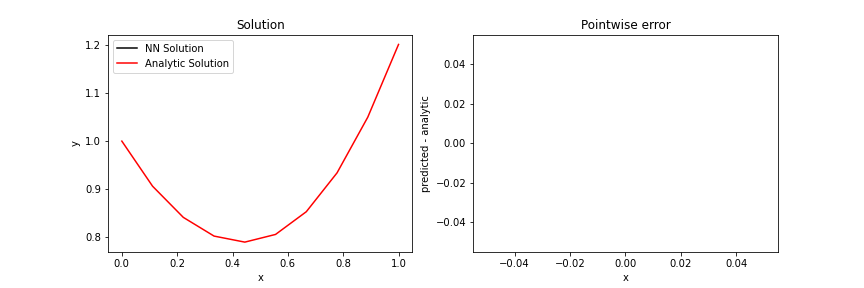
\includegraphics[scale=0.6]{code/train.png} \\
        Figure 1: Results of training the network using $\tanh$ with default settings.
    \end{center}
    
    \begin{center}
        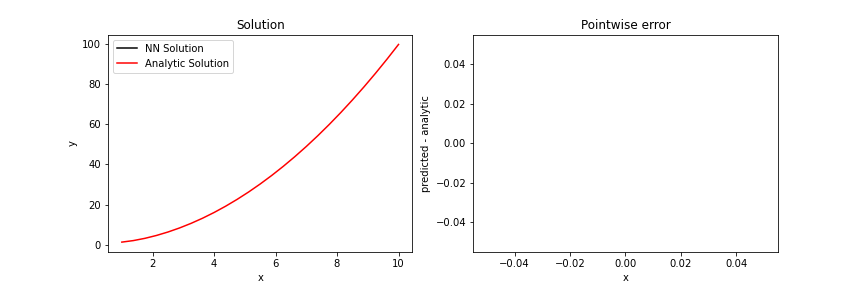
\includegraphics[scale=0.6]{code/predict.png} \\
        Figure 2: Results of training the network using $\tanh$ with default settings.
    \end{center}
    
    After that, I tested out the three activation functions to see if they made a difference. From there, I learned I should have actually been using a ReLU activation the whole time (Figure 3)! 

    I tried adding another layer but have as of yet been unsuccessful---there are some implementation details I have yet to work out. The attached code has the beginnings of my attempt, however.
    
    \begin{center}
        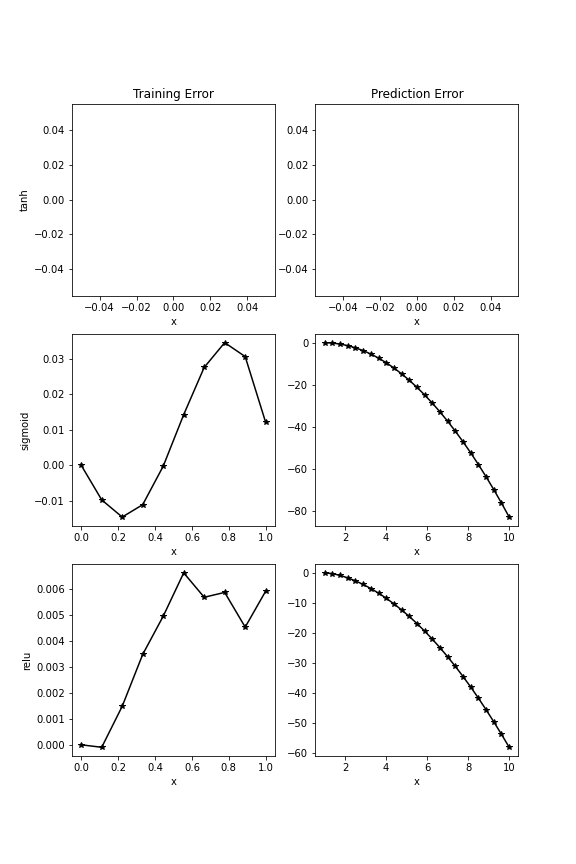
\includegraphics[scale=0.75, trim={0cm 2cm 2cm 2cm}, clip]{code/activations.png} \\
        Figure 3: Training and prediction error for various activation functions. Note that the $y$ axes are all different.
    \end{center}}
\end{document}